\subsection{MSVC + \olly}
\index{\olly}
\RU{Проиллюстрируем всё это в}\EN{Let's illustrate this in} \olly.
\RU{Когда мы протрассируем до первой инструкции в \ttf, которая использует какой-то из аргументов
(первый), мы увидим, что \EBP указывает на \glslink{stack frame}{фрейм стека}. Он выделен красным прямоугольником.}%
\EN{When we trace to the first instruction in \ttf that uses one of the arguments 
(first one), we see that \EBP is pointing to the \gls{stack frame}, 
which is marked with a red rectangle.}
\RU{Самый первый элемент \glslink{stack frame}{фрейма стека}~--- это сохраненное значение \EBP, 
затем \ac{RA}. Третий элемент это первый аргумент функции, затем второй аргумент и третий.}
\EN{The first element of the \gls{stack frame} is the saved value of \EBP, 
the second one is \ac{RA}, the third is the first function argument, then the second and third ones.}
\RU{Для доступа к первому аргументу функции нужно прибавить к \EBP 8 (2 32-битных слова).}
\EN{To access the first function argument, one needs to add exactly 8 (2 32-bit words) to \EBP.}

\olly \EN{is aware about this, so it has added comments to the stack elements like}
\RU{в курсе этого, так что он добавил комментарии к элементам стека вроде}
\q{RETURN from} \AndENRU \q{Arg1 = \dots}, \etc{}.

N.B.: \EN{Function arguments are not members of the function's stack frame, they are rather
members of the stack frame of the \gls{caller} function.}
\RU{аргументы функции являются членами фрейма стека вызывающей функции, а не текущей.}
\EN{Hence, \olly marked \q{Arg} elements as members of another stack frame.}
\RU{Поэтому \olly отметил элементы \q{Arg} как члены другого фрейма стека.}

\begin{figure}[H]
\centering
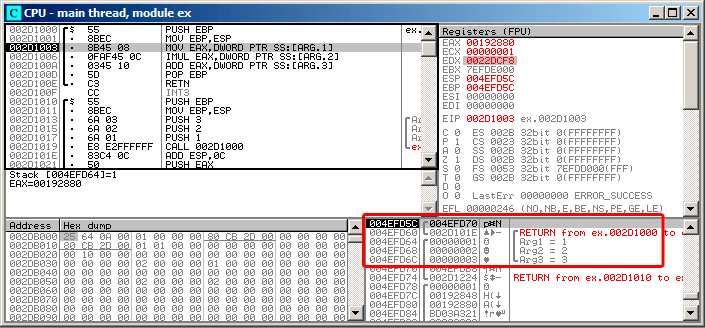
\includegraphics[scale=\FigScale]{patterns/05_passing_arguments/olly.png}
\caption{\olly: \RU{внутри функции}\EN{inside of} \ttf{}\EN{ function}}
\label{fig:passing_arguments_olly}
\end{figure}
